\lecture{24}{21. November 2024}{Fluiddynamik}
Sidst blev der arbejdet med stillestående væsker. I dag udvider vi dette til også at inkludere en hastighed. 

\begin{figure} [ht]
  \centering
  \caption{Tegning af en inkompressibel væske i bevægelse fra bogen.}
  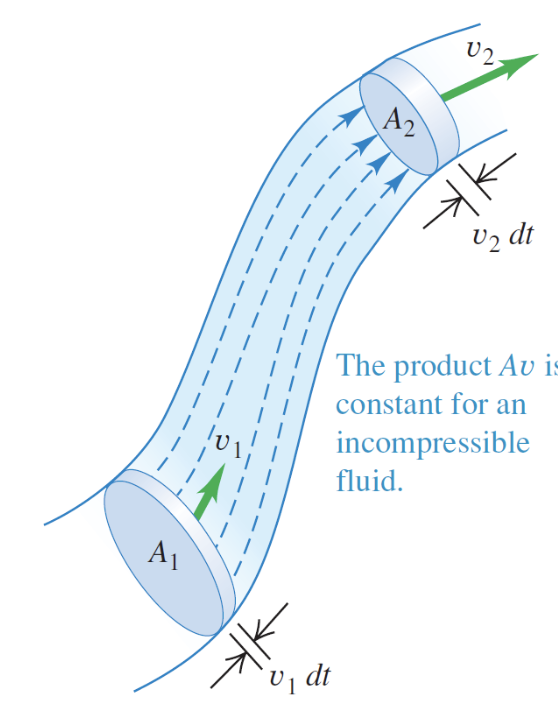
\includegraphics[width=0.3\linewidth]{./figures/F24_12_4.png}
  \label{fig:F24_12_4}
\end{figure}

Vi antager, at alle væsker vi kommer til at arbejde med i det følgende er inkopressible. På \textbf{\autoref{fig:F24_12_4}} ses en inkompressibel væske i bevægelse. Idet væsken er inkompressibel gælder følgende 
\begin{align*}  
  \, \mathrm{d}m_1 &= \, \mathrm{d}m_2  \\
  \rho \, \mathrm{d}V_1 &= \rho \, \mathrm{d}V_2 \\
  \\
  \rho A_1v_1 \, \mathrm{d}t &= \rho A_2 v_2 \, \mathrm{d}t  \\
  &\Downarrow \\
  A_1 v_1 &= A_2 v_2 \\
  A v &= \mathrm{const.}
.\end{align*} 

Det sidste udtryk fra ovenfor kaldes ofte \textit{kontinuitetslignignen}. 
\begin{sæt}[kontinuitetslignignen]
  Vi har generelt for inkompressible væsker, at
  \[ 
    A v = \mathrm{const.}
  .\]
\end{sæt}

\section{Arbejdet på væsken}
Vi har generelt at
\[ 
\rho \, \mathrm{d}V_1 = \rho A_1 v_1 \, \mathrm{d}t \implies \frac{\mathrm{d}V}{\mathrm{d}t} = Av
.\]
Det ovenstående kan nu omskrives som
\begin{align*}
  \, \mathrm{d}V &= A_1 \, \mathrm{d}s_1 = A_2 \, \mathrm{d}s_2
.\end{align*}
Derfor er arbejdet udført på væsken
\[ 
  \, \mathrm{d}W = P_1 \underbrace{A_1 \, \mathrm{d}s_1}_{\mathrm{d}V} - P_2 \underbrace{A_2 \, \mathrm{d}s_2}_{\mathrm{d}V} = (P_1 - P_2)\, \mathrm{d}V
.\]

\section{Kinetisk energi}
Den kinetiske energi af volumenet af væsken der ``flyder ind'' er
\[ 
\mathrm{d}K_1 = \frac{1}{2} \, \mathrm{d}m_1 v_1^2 = \frac{1}{2}(\rho A_1 \, \mathrm{d}s_1) v_1^2 = \frac{1}{2}\rho \, \mathrm{d}V v_1^2
.\]
Og den kinetiske energi af volumenet af væsken der ``flyder ud'' er
\[ 
\mathrm{d}K_2 = \frac{1}{2} \, \mathrm{d}m_2 v_2^2 = \frac{1}{2}(\rho A_2 \, \mathrm{d}s_2) v_2^2 = \frac{1}{2}\rho \, \mathrm{d}V v_2^2
.\]
Ændringen i kinetisk energi er da
\begin{align*}
  \Delta K &= \, \mathrm{d}K_2 - \, \mathrm{d}K_1 \\
  &= \frac{1}{2}\rho \, \mathrm{d}V \left( v_2^2 - v_1^2 \right)
.\end{align*}

\section{Ændringen i potentiel energi}
Vi har at
\[ 
  \underbrace{\mathrm{d}m_1}_{\text{Massen der flyder ind}} = \underbrace{\mathrm{d}m_2}_{\text{Massen der flyder ud}} = \, \mathrm{d}m
.\]

Den potentielle energi for væsken der flyder ind er da
\[ 
  \mathrm{d}U_1 = \, \mathrm{d}m g y_1 = \rho \, \mathrm{d}V g y_1
.\]

Og den potentielle energi for den del af væsken der flyder ud er
\[ 
    \mathrm{d}U_2 = \, \mathrm{d}m g y_2 = \rho \, \mathrm{d}V g y_2
.\]

Så ændringen er altså
\[ 
  \mathrm{d}U = \mathrm{d}U_2 - \mathrm{d}U_1 = \rho \, \mathrm{d}V g (y_2 - y_1)
.\]

\subsection{Det tilførte arbejde}
Tilført arbejde er lig ændringen i mekanisk energi. Altså
\[ 
  \, \mathrm{d}W = \mathrm{d}E = \, \mathrm{d}K + \, \mathrm{d}U
.\]
Hvis vi indsætter de tidligere udledte udtryk fås, at
\begin{align*}
  (P_1 - P_2) \, \mathrm{d}V & = \frac{1}{2}\rho \, \mathrm{d}V \left( v_2^2 - v_1^2 \right) + \rho \, \mathrm{d}V g(y_2 - y_1)  \\
  (P_1 - P_2) &= \frac{1}{2}\rho \left( v_2^2 - v_1^2 \right) + \rho g (y_2 - y_1)  \\
  P_1 + \frac{1}{2}\rho v_1^2 + \rho g y_1 &= P_2 + \frac{1}{2}\rho v_2^2 + \rho g y_2
.\end{align*}

\begin{sæt}[Bernoullis ligning]
  Idet udtrykket fundet ovenfor gælder for alle punkter i væsken kan vi skrive det som
  \[ 
    P + \frac{1}{2}\rho v^2 + \rho g y = \mathrm{const}
  .\]
  Denne sammenhæng kaldes Bernoullis ligning og den gælder for væsker hvor følgende antagelser er valide
  \begin{itemize}
    \item \textbf{Inkompressibel}: En ændring i trykket medfører ikke en ændring i volumen.
    \item \textbf{Inviskos}: Væsken har ingen indre friktion
    \item \textbf{Stationær strømning}: Væskens hastighed er konstant ($\frac{\mathrm{d}V^2}{\mathrm{d}t} = 0$)
  \end{itemize}
\end{sæt}

\begin{eks}[Udstrømningshastighed (12.8)]
  Vi betragter en stor oliebeholder. Oliebeholderen har en iregulær form og vi ønsker, at finde udstrømningshastigehden for væsken i beholderen. Trykket over væskespejlet indeni beholderen betegnes, $p_0$, arealet af væskespejlet i toppen betegnes $A_1$, arealet af ``væskespejlet'' i bunden betegnes $A_2$ og trykket lige uden for punktet hvor væsken udstrømmer fra betegnes $p_{atm}$. Vi kan bruge Bernoullis ligning som
  \[ 
  p_0 + \underbrace{\frac{1}{2} \rho v_1^2}_{\approx 0, \text{ da } (A_1 \gg A_2)} + \rho gh = p_{atm} + \frac{1}{2} \rho v_2^2 + 0
  .\]
  Vi får da
  \[ 
  v_2^2 = \frac{2}{\rho}(p_0 - p_{atm}) + 2gh
  .\]
  Hvis beholderen, var åben i toppen således at $p_0 = p_{atm}$ så får vi
  \[ 
  v_2 = \sqrt{2gh}
  .\]
  Hvilket blot er den almindelige hastighed for et frit fald.
\end{eks}

